%%%%%%%%%%%%%%%%%%%%%%%%%%%%%%%%%%%%%%%%%%%%%%%%%%%%%%%%%%%%%%%%%%%%%%%%%%%%%%%%
%%% main document {{{

\documentclass[
a4paper,     %% defines the paper size: a4paper (default), a5paper, letterpaper, ...
% landscape,   %% sets the orientation to landscape
% twoside,     %% changes to a two-page-layout (alternatively: oneside)
% twocolumn,   %% changes to a two-column-layout
 headsepline, %% add a horizontal line below the column title
 footsepline, %% add a horizontal line above the page footer
 titlepage,   %% only the titlepage (using titlepage-environment) appears on the first page (alternatively: notitlepage)
% halfparskip,     %% insert an empty line between two paragraphs (alternatively: halfparskip, ...)
% leqno,       %% equation numbers left (instead of right)
 fleqn,       %% equation left-justified (instead of centered)
% tablecaptionabove, %% captions of tables are above the tables (alternatively: tablecaptionbelow)
% draft,       %% produce only a draft version (mark lines that need manual edition and don't show graphics)
12pt         %% set default font size
]{scrartcl}  %% article, see KOMA documentation (scrguide.dvi)

%%%%%%%%%%%%%%%%%%%%%%%%%%%%%%%%%%%%%%%%%%%%%%%%%%%%%%%%%%%%%%%%%%%%%%%%%%%%%%%%
%%%
%%% packages
%%%
\usepackage[a4paper, bottom=3cm, top=3cm]{geometry}

%%% babel: language set (can cause some conflicts with package ngerman)
%%%        use it only for multi-language documents or non-german ones
\usepackage[english]{babel}

%%% inputenc: coding of german special characters
\usepackage[latin1]{inputenc}

%%% fontenc, ae, aecompl: coding of characters in PDF documents
\usepackage[T1]{fontenc}
\usepackage{ae,aecompl}

%%%
%%% technical packages
%%%

%%% amsmath, amssymb, amstext: support for mathematics
\usepackage{amsmath,amssymb,amstext}

%%% psfrag: replace PostScript fonts
%\usepackage{psfrag}

%%% listings: include programming code
%\usepackage{listings}

%%% units: technical units
\usepackage{units}

%%%
%%% layout
%%%

%%% scrpage2: KOMA heading and footer
%%% Note: if you don't use this package, please remove 
%%%       \pagestyle{scrheadings} and corresponding settings
%%%       below too.
\usepackage{scrpage2}

\usepackage{titlepic}

%%%
%%% PDF
%%%

%\newif\ifpdf
%  \ifx\pdfoutput\undefined
%     \pdffalse
%  \else
%     \pdfoutput=1
%     \pdftrue
%  \fi

%%% Should be LAST usepackage-call!
%%% For docu on that, see reference on package ``hyperref''
\ifpdfoutput{%   (definitions for using pdflatex instead of latex)

  %%% graphicx: support for graphics
  \usepackage[pdftex]{graphicx}

  \pdfcompresslevel=9

  %%% hyperref (hyperlinks in PDF): for more options or more detailed
  %%%          explanations, see the documentation of the hyperref-package
  \usepackage[%
    %%% general options
    %pdftex=true,      %% sets up hyperref for use with the pdftex program
    %plainpages=false, %% set it to false, if pdflatex complains: ``destination with same identifier already exists''
    %
    %%% extension options
    %backref=true,      %% if true, adds a backlink text to the end of each item in the bibliography
    pagebackref=false, %% if true, creates backward references as a list of page numbers in the bibliography
    colorlinks=true,   %% turn on colored links (true is better for on-screen reading, false is better for printout versions)
    %
    %%% PDF-specific display options
    bookmarks=true,          %% if true, generate PDF bookmarks (requires two passes of pdflatex)
    bookmarksopen=false,     %% if true, show all PDF bookmarks expanded
    bookmarksnumbered=false, %% if true, add the section numbers to the bookmarks
    %pdfstartpage={1},        %% determines, on which page the PDF file is opened
    pdfpagemode=UseNone         %% None, UseOutlines (=show bookmarks), UseThumbs (show thumbnails), FullScreen
  ]{hyperref}


  %%% provide all graphics (also) in this format, so you don't have
  %%% to add the file extensions to the \includegraphics-command
  %%% and/or you don't have to distinguish between generating
  %%% dvi/ps (through latex) and pdf (through pdflatex)
  \DeclareGraphicsExtensions{.pdf}

}{%else   (definitions for using latex instead of pdflatex)

  \usepackage[dvips]{graphicx}

  \DeclareGraphicsExtensions{.eps}

  \usepackage[%
    dvips,           %% sets up hyperref for use with the dvips driver
    colorlinks=false %% better for printout version; almost every hyperref-extension is eliminated by using dvips
  ]{hyperref}

}


%%% sets the PDF-Informations options
%%% (see fields in Acrobat Reader: ``File -> Document properties -> Summary'')
%%% Note: this method is better than as options of the hyperref-package (options are expanded correctly)
\hypersetup{
  pdftitle={MaGrav Power System - Construction Manual}, %%
  pdfauthor={}, %%
  pdfsubject={}, %%
  pdfcreator={Accomplished with LaTeX2e and pdfLaTeX with hyperref-package.}, %% 
  pdfproducer={}, %%
  pdfkeywords={} %%
}


%%%%%%%%%%%%%%%%%%%%%%%%%%%%%%%%%%%%%%%%%%%%%%%%%%%%%%%%%%%%%%%%%%%%%%%%%%%%%%%%
%%%
%%% user defined commands
%%%

%%% \mygraphics{}{}{}
%% usage:   \mygraphics{width}{filename_without_extension}{caption}
%% example: \mygraphics{0.7\textwidth}{rolling_grandma}{This is my grandmother on inlinescates}
%% requires: package graphicx
%% provides: including centered pictures/graphics with a boldfaced caption below
%% 
\newcommand{\mygraphics}[3]{
  \begin{center}
    \includegraphics[width=#1, keepaspectratio=true]{#2} \\
    \textbf{#3}
  \end{center}
}

%%%%%%%%%%%%%%%%%%%%%%%%%%%%%%%%%%%%%%%%%%%%%%%%%%%%%%%%%%%%%%%%%%%%%%%%%%%%%%%%
%%%
%%% define the titlepage
%%%



%\makeatother
% \publishers{}
% \thanks{} %% use it instead of footnotes (only on titlepage)
% \dedication{} %% generates a dedication-page after titlepage


%%% uncomment following lines, if you want to:
%%% reuse the maketitle-entries for hyperref-setup
%\newcommand\org@maketitle{}
%\let\org@maketitle\maketitle
%\def\maketitle{%
%  \hypersetup{
%    pdftitle={\@title},
%    pdfauthor={\@author}
%    pdfsubject={\@subject}
%  }%
%  \org@maketitle
%}


%%%%%%%%%%%%%%%%%%%%%%%%%%%%%%%%%%%%%%%%%%%%%%%%%%%%%%%%%%%%%%%%%%%%%%%%%%%%%%%%
%%%
%%% set heading and footer
%%%

%%% scrheadings default: 
%%%      footer - middle: page number
\pagestyle{scrheadings}

%%% user specific
%%% usage:
%%% \position[heading/footer for the titlepage]{heading/footer for the rest of the document}

%%% heading - left
% \ihead[]{}

%%% heading - center
% \chead[]{}

%%% heading - right
 \ohead[]{MaGrav Power Supply - Construction Manual}

%%% footer - left
% \ifoot[]{}

%%% footer - center
% \cfoot[]{}

%%% footer - right
% \ofoot[]{}



%%%%%%%%%%%%%%%%%%%%%%%%%%%%%%%%%%%%%%%%%%%%%%%%%%%%%%%%%%%%%%%%%%%%%%%%%%%%%%%%
%%%
%%% begin document
%%%

\begin{document}

\subject{MaGrav Power Supply}
\title{Construction Manual}
\author{Knowledge Seeker(s)}
\date{Earth, \today}

\begin{titlepage}
	\centering
	
\includegraphics[width=0.40\textwidth]{images/kf_ssi_logo.jpg}\par
	\vspace{3cm}
	{\scshape\LARGE Keshe Foundation Space Ship Institute \par}
	\vspace{1cm}
	{\scshape\large MaGrav Power Supply\par}
	\vspace{1.5cm}
	{\huge\bfseries Construction Manual\par}
	\vspace{2cm}
	{\large\itshape Knowledge Seeker(s)\par}
	\vfill


% Bottom of the page
	{Earth, \today \par}
\end{titlepage}



%%% include the title
 % \thispagestyle{empty}  %% no header/footer (only) on this page
 % \maketitle

 \pagenumbering{roman} %% small roman page numbers

%%% start a new page and display the table of contents
 % \newpage
 \tableofcontents

%%% start a new page and display the list of figures
 \newpage
 \listoffigures

%%% start a new page and display the list of tables
% \newpage
 \listoftables

%%% display the main document on a new page 
 \newpage

 \pagenumbering{arabic} %% normal page numbers (include it, if roman was used above)

%%%%%%%%%%%%%%%%%%%%%%%%%%%%%%%%%%%%%%%%%%%%%%%%%%%%%%%%%%%%%%%%%%%%%%%%%%%%%%%%
%%%
%%% begin main document
%%% structure: \section \subsection \subsubsection \paragraph \subparagraph
%%%

\section*{Introduction or Foreword}
\label{sec:introduction}


This is a placeholder for the introduction.

\newpage

\section{Disclaimer}
\label{sec:disclaimer}

\section{Required components}
\label{sec:required-components}

\subsection{Global list of suppliers}
\label{sec:global-list-of-suppliers}

\begin{table}[h]
\begin{center}
    \begin{tabular}{ | l | l |} \hline
    Component & Supplier \\ \hline
    Bare Copper Wire, Bright, 14 AWG, 0.064" Diameter, 80' Length  &  
    \href{http://www.amazon.com/Copper-Bright-0-064-Diameter-Length/dp/B000IJYRDE/ref=sr_1_15?ie=UTF8&qid=1446585445&sr=8-15&keywords=awg+14+copper}{Amazon}  \\ \hline

    \end{tabular}
    \caption{Global list of suppliers}
	\label{table:global-list-suppliers}
\end{center}
\end{table}

\section{Required assembly tools}
\label{sec:required-assembly-tools}

\subsection{Global list of vendors}
\label{sec:global-list-of-vendors}

\section{Assembly}
\label{sec:assembly}

\subsection{Coils}
\label{sec:coils}

\begin{figure}[h]
  \centering
  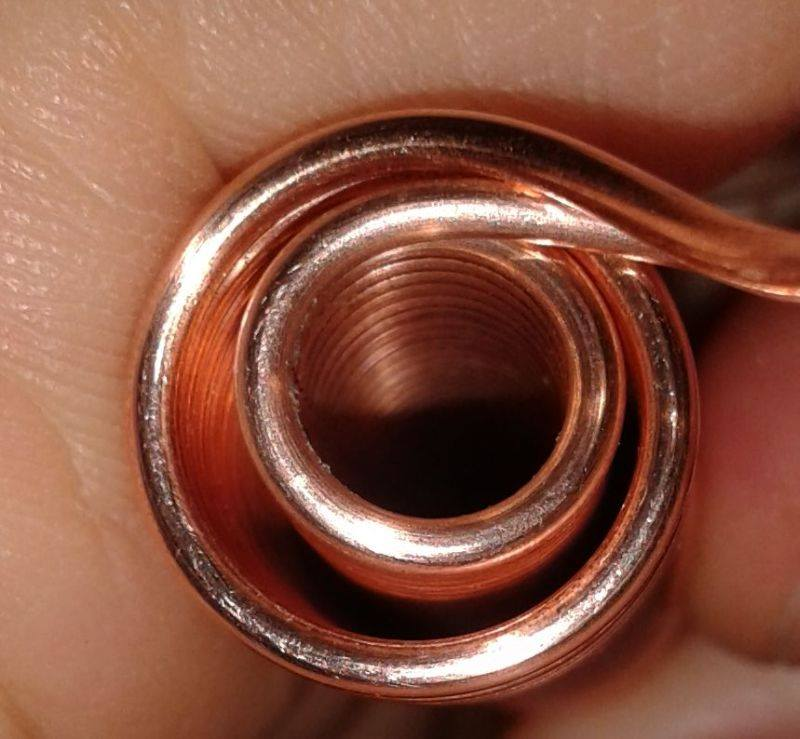
\includegraphics[width=50mm]{images/counter_clock_wise_winding.jpg}
  \caption[Counter-clock-wise (CCW) winding of a copper coil]{Counter-clock-wise (CCW) winding of a copper coil}
  \label{fig:ccw}
\end{figure}

\subsection{Coils casings}
\label{sec:coils-casings}

\subsection{Coils hinges}
\label{sec:coils-hinges}

\subsection{Internal wiring}
\label{sec:internal-wiring}

\subsection{MaGrav shell}
\label{sec:magrav-shell}

\subsection{Box}
\label{sec:box}

\subsubsection{Wall socket}
\label{sec:wall-socket}

\section{Support resources}


%\begin{figure}[bt]
%  \centering
%  \includegraphics{./images/nameofimage}
%  \caption[example caption]{example caption}
%  \label{fig:schema}
%\end{figure}



%%%
%%% end main document
%%%
%%%%%%%%%%%%%%%%%%%%%%%%%%%%%%%%%%%%%%%%%%%%%%%%%%%%%%%%%%%%%%%%%%%%%%%%%%%%%%%%

 \appendix  %% include it, if something (bibliography, index, ...) follows below

%%%%%%%%%%%%%%%%%%%%%%%%%%%%%%%%%%%%%%%%%%%%%%%%%%%%%%%%%%%%%%%%%%%%%%%%%%%%%%%%
%%%
%%% bibliography
%%%
%%% available styles: abbrv, acm, alpha, apalike, ieeetr, plain, siam, unsrt
%%%
 \bibliographystyle{plain}

%%% name of the bibliography file
 \bibliography{project.bib}

\end{document}
%%% }}}
%%% END OF FILE
%%%%%%%%%%%%%%%%%%%%%%%%%%%%%%%%%%%%%%%%%%%%%%%%%%%%%%%%%%%%%%%%%%%%%%%%%%%%%%%%
%% Local Variables:
%% mode: outline-minor
%% OPToutline-regexp: "%% .*"
%% OPTeval: (hide-body)
%% emerge-set-combine-versions-template: "%a\n%b\n"
%% End:
%% vim:foldmethod=marker
